\documentclass{beamer}
\usepackage{graphicx}
\usepackage{amsmath,amssymb,amstext,amsthm,xargs}
\usepackage{amsfonts}
\usepackage{bbm}
\usepackage{beamerthemesplit}

\usepackage[utf8]{inputenc}
\usepackage[french]{babel}
\usepackage{bbm}

\usetheme{Antibes}
\mode<presentation>
\useoutertheme{tree}
\usecolortheme{beaver}
\useinnertheme{rectangles}

\setbeamerfont{block title}{size={}}
%\usecolortheme[rgb={0.55,0.1,0.05}]{structure}
%\usecolortheme[rgb={0.75,0.1,0.05}]{structure}
\usepackage{color}

\newenvironment{disarray}{\everymath{\displaystyle\everymath{}}\array} {\endarray}
\newtheorem{theo}{Théorème}
\newtheorem{prop}[theo]{Proposition}
\newtheorem{conj}[theo]{Conjecture}
\newtheorem{cor}{Corollary}[theo]

\newtheorem{lem}{Lemme}
\newtheorem{nota}{Notation}
\newtheorem{rk}{Remark}
\newtheorem{exa}{Example}
\newtheorem{df}{Definition}
\newtheorem{terminologie}{Terminologie}
\def\rme{\mathrm{e}}
\def\rmi{\mathrm{i}}
\def\rset{\mathbb{R}}
\def\nset{\mathbb{N}}
\def\dlim{\stackrel{d}{\rightarrow}}
\newcommandx{\plim}[1][1=]{\stackrel{\PP_{#1}}{\longrightarrow}}
\def\iid{i.i.d.}
\def\1{\mathbbm{1}}
\newenvironment{dem}{\textbf{Proof}}{\flushright$\blacksquare$\\}
%\def\blankframe{
%\mode<presentation>{
%  { \setbeamertemplate{background canvas}[default]
%    \setbeamercolor{background canvas}{bg=black}
%    \begin{frame}[plain]{}
%    \end{frame}
%  }
%}
%\mode<presentation>{
%\setbeamertemplate{background canvas}[default]
%\setbeamercolor{background canvas}{bg=white}}
%\mode*
%}
\def\eqsp{\,}
\DeclareMathOperator{\E}{{\mathbb E}}
\def\PE{\E}
\def\PCov{\mathrm{Cov}}
\DeclareMathOperator{\F}{{\mathbb F}}
\DeclareMathOperator{\G}{{\mathbb G}}
\DeclareMathOperator{\D}{{\mathbb D}}
\DeclareMathOperator{\R}{{\mathbb R}}
\DeclareMathOperator{\C}{{\mathbb C}}
\DeclareMathOperator{\Z}{{\mathbb Z}}
\DeclareMathOperator{\N}{{\mathbb N}}
\DeclareMathOperator{\K}{{\mathbb K}}
\DeclareMathOperator{\T}{{\mathbb T}}
\DeclareMathOperator{\PP}{{\mathbb P}}
\DeclareMathOperator{\QQ}{{\mathbb Q}}
\DeclareMathOperator{\Q}{{\mathbb Q}}
\DeclareMathOperator{\IF}{{\mathbb I}}


%%%%%%%%%%%%%%%%%%%%%%%%%%%%%%% Pour le modèle lin\'eaire

\DeclareMathOperator{\bX}{\boldsymbol{X}}
\DeclareMathOperator{\bY}{\boldsymbol{Y}}
\DeclareMathOperator{\bx}{\boldsymbol{x}}
\DeclareMathOperator{\vp}{\boldsymbol{p}}
\DeclareMathOperator{\vq}{\boldsymbol{q}}
\DeclareMathOperator{\estMCNL}{\widehat \theta_n^{\,\,{\tt mcnl}}}
\DeclareMathOperator{\estMV}{\widehat \theta_n^{\,\,{\tt mv}}}
\DeclareMathOperator{\est}{\widehat \theta_{\mathnormal{n}}}
\DeclareMathOperator{\var}{\mathrm{Var}}
\def\Var{\var}
\DeclareMathOperator{\estMVc}{\widehat \theta_{n,0}^{\,{\tt mv}}}
\DeclareMathOperator{\Xbar}{\overline{\mathnormal{X}}_\mathnormal{n}}

\newcommand{\indi}[1]{\mathbbm{1}_{\{#1\}}}
\newcommand{\coint}[1]{\left[#1\right)}
\newcommand{\ocint}[1]{\left(#1\right]}
\newcommand{\ooint}[1]{\left(#1\right)}
\newcommand{\ccint}[1]{\left[#1\right]}

\definecolor{LightYell}{rgb}{0.95,0.83,0.70}
\definecolor{orange}{rgb}{1.0,0.50,0.01}
\definecolor{StroYell}{rgb}{0.95,0.88,0.72}
\definecolor{lightred}{rgb}{0.75,0.033,0}
\definecolor{shadecolor1}{rgb}{0.90,0.83,0.70}
\definecolor{myem}{rgb}{0.797,0.598,0.598}
\definecolor{BrickRed}{cmyk}{0,0.89,0.94,0.28}
\definecolor{RoyalPurple}{cmyk}{0.75,0.9,0,0}

\newcommand{\tco}[1]{\textcolor{orange}{#1}}
\newcommand{\tcr}[1]{\textcolor{lightred}{#1}}

\def\gauss{\mathcal{N}}
\def\truetheta{\theta}
\def\truebeta{\boldsymbol{\beta}}
\def\projX{A}
\def\curtheta{\alpha}
\def\argmin{\mathrm{argmin}}
\def\ie{\emph{i.e.}}
\def\regressmat{\mathbb{X}}
\def\errpred{\boldsymbol{\hat{\xi}}}
\def\bnoise{\boldsymbol{\xi}}
\def\predY{\hat{\mathbf{Y}}}
\DeclareMathOperator{\estregress}{\widehat{\truebeta}_n}
\DeclareMathOperator{\estMC}{\widehat \theta_n^{\,\,{\tt mc}}}
\def\curbeta{b}
\def\bcurbeta{\mathbf{b}}
\newcommand{\indep}{\rotatebox[origin=c]{90}{$\models$}} 
\newcommand{\Id}[1]{\mathrm{Id}_{#1}}

\title{MAP 433 : Introduction aux méthodes statistiques. Cours 6}
%\author{M. Hoffmann}
%\institute{Université Paris Dauphine}

\begin{document}
\date{2 Octobre 2015}
\maketitle



\begin{frame}
\frametitle{Aujourd'hui}
\tableofcontents
\end{frame}


\section{Tests statistiques}

\subsection{Notion de test et d'erreur de test}



\begin{frame}
\frametitle{Exemple introductif}
\begin{itemize}
\item On observe 10 lancers d'une pièce de monnaie et on obtient le résultat suivant :
$$(P, P, F, F, P, F, P, P, F, P).$$
\alert{La pièce est-elle équilibrée} ?
\item \alert{Répondre} à cette question revient à \alert{construire une procédure de décision} :
$$\varphi = \varphi(P, P, F, F, P, F, P, P, F, P)$$
$$ =
\left\{
\begin{array}{ll}
0 & \text{\alert{on accepte} l'hypothèse  la pièce est équilibrée} \\
1 & \text{\alert{on rejette} l'hypothèse  la pièce est équilibrée}
\end{array}
\right.$$
\end{itemize}
\end{frame}

\begin{frame}
\frametitle{Résolution}
\begin{itemize}
\item On associe l'expérience statistique (par exemple)
$${\mathcal E}^{10} = \big(\{0,1\}^{10}, \text{{\small parties de}}(\{0,1\}^{10}), \{\PP_\truetheta^{10}, \truetheta \in \Theta = [0,1]\}\big),$$
avec ($P=0$, $F=1$)
$$\PP^{10}_\truetheta=\big(\truetheta\delta_{0}(dx)+(1-\truetheta)\delta_{1}(dx)\big)^{\otimes 10}.$$
\item\underline{Hypothèse nulle} :  \alert{  la pièce est équilibrée }
$$\boxed{H_0: \truetheta \in \Theta_0 = \{ 1/2\} }$$
\item \underline{Hypothèse alternative} :  \alert{ la pièce est truquée}
$$\boxed{H_1 : \truetheta \in \Theta_1 = \Theta \setminus \{1/2\}}$$
\end{itemize}
\end{frame}

\begin{frame}
\frametitle{Résolution}
\begin{itemize}
\item $\Theta_0$= ensemble des paramètres sous laquelle l'hypothèse nulle est satifaite
\item $\Theta_1$= ensemble des paramètres sous laquelle l'hypothèse nulle n'est pas satisfaite = \alert{alternative}
\item $\Theta= \Theta_0 \cup \Theta_1$.
\end{itemize}
\end{frame}

\begin{frame}
\frametitle{Règle de décision}
\begin{itemize}
\item On note $Z$ l'observation.
\item On \alert{construit} une \alert{règle de décision simple} :
$$\varphi(Z) = \1_{\zreject}(Z) =
\begin{cases}
0 & \text{on accepte l'hypothèse} \\
1 & \text{on rejette l'hypothèse.}
\end{cases}
$$
\item $ \zreject\subset {\mathfrak Z}$ (espace des observables) : \alert{zone de rejet} ou \alert{région critique}.
\item \underline{Exemple}\footnote{léger abus de notation...}
$$\zreject = \big\{\big|\widehat \truetheta(z)-1/2\big| > t_0\big\},\;\;\widehat \truetheta(Z) = \estMV \big(\stackrel{exemple}{=} 0,6\big)$$
où $t_0$ est un seuil à choisir... \alert{Comment ?}
\end{itemize}
\end{frame}

\begin{frame}
\frametitle{Terminologie}
\begin{itemize}
\item Une \alert{règle de décision} (non-randomisée) assigne à chaque réalisation $z$ de l'observation $Z$ une \alert{décision}.
\item Si $z \in \zaccept$, l'hypothèse nulle est \alert{acceptée}; autrement, l'hypothèse est rejetée.
\item \alert{Terminologie}: $\zaccept$= \alert{zone d'acceptation} ; $\zreject$= \alert{zone de rejet} ou \alert{région critique}.
\end{itemize}
\end{frame}

\begin{frame}
\frametitle{Erreur de décision}
\begin{itemize}
\item
Lorsque l'on prend la décision $\varphi(Z)$, on peut se \alert{tromper de deux manières} :
$$\text{\alert{Rejeter}}\; H_0\;\;(\varphi(Z)=1)\;\;\text{\alert{alors que}}\;\;\truetheta = \frac{1}{2}$$
ou encore
$$\text{\alert{Accepter}}\;H_0\;\;(\varphi(Z)=0)\;\;\text{\alert{alors que}}\;\;\truetheta  \neq \frac{1}{2}.$$
\item \underline{Erreur de première espèce}  \alert{(=rejeter à tort)}
$$\PP_{\tfrac{1}{2}}^{10}\big[\varphi(Z)=1\big]$$
\item \underline{Erreur de seconde espèce}  \alert{(=accepter à tort)}
$$\big(\PP_\truetheta^{10}\big[\varphi(Z)=0\big],\;\;\truetheta \neq \frac{1}{2}\big).$$
\end{itemize}
\end{frame}


\begin{frame}
\frametitle{Retour à l'exemple}
\begin{itemize}
\item Sous $\PP_\theta$, $n \hat{\theta}(Z)= \sum_{i=1}^n Z_i$ suit une loi binomiale de paramètre de succès $\truetheta$. 
En notant $\binom_{n,\truetheta}$ la fonction
de répartition de la loi binomiale,
\begin{multline*}
\PP_\truetheta( |\hat{\theta}(Z) - 1/2| > t_0 ) \\
= 1 - \{\binom_{n,\truetheta}(n(1+t_0)/2) - \binom_{n,\truetheta}(n(1-t_0)/2)  \} \eqsp.
\end{multline*}
\item \alert{Erreur de première espèce}:
\begin{multline*}
\PP_{1/2}(|\hat{\theta}(Z) - 1/2| > t_0) \\= 1 - \{ \binom_{n,1/2}(n(1+t_0)/2) - \binom_{n,1/2}(n(1-t_0)/2)  \}
\end{multline*}
\end{itemize}
\end{frame}

\begin{frame}
\frametitle{Erreur de première espèce}
\begin{figure}
  \centering
  % Requires \usepackage{graphicx}
  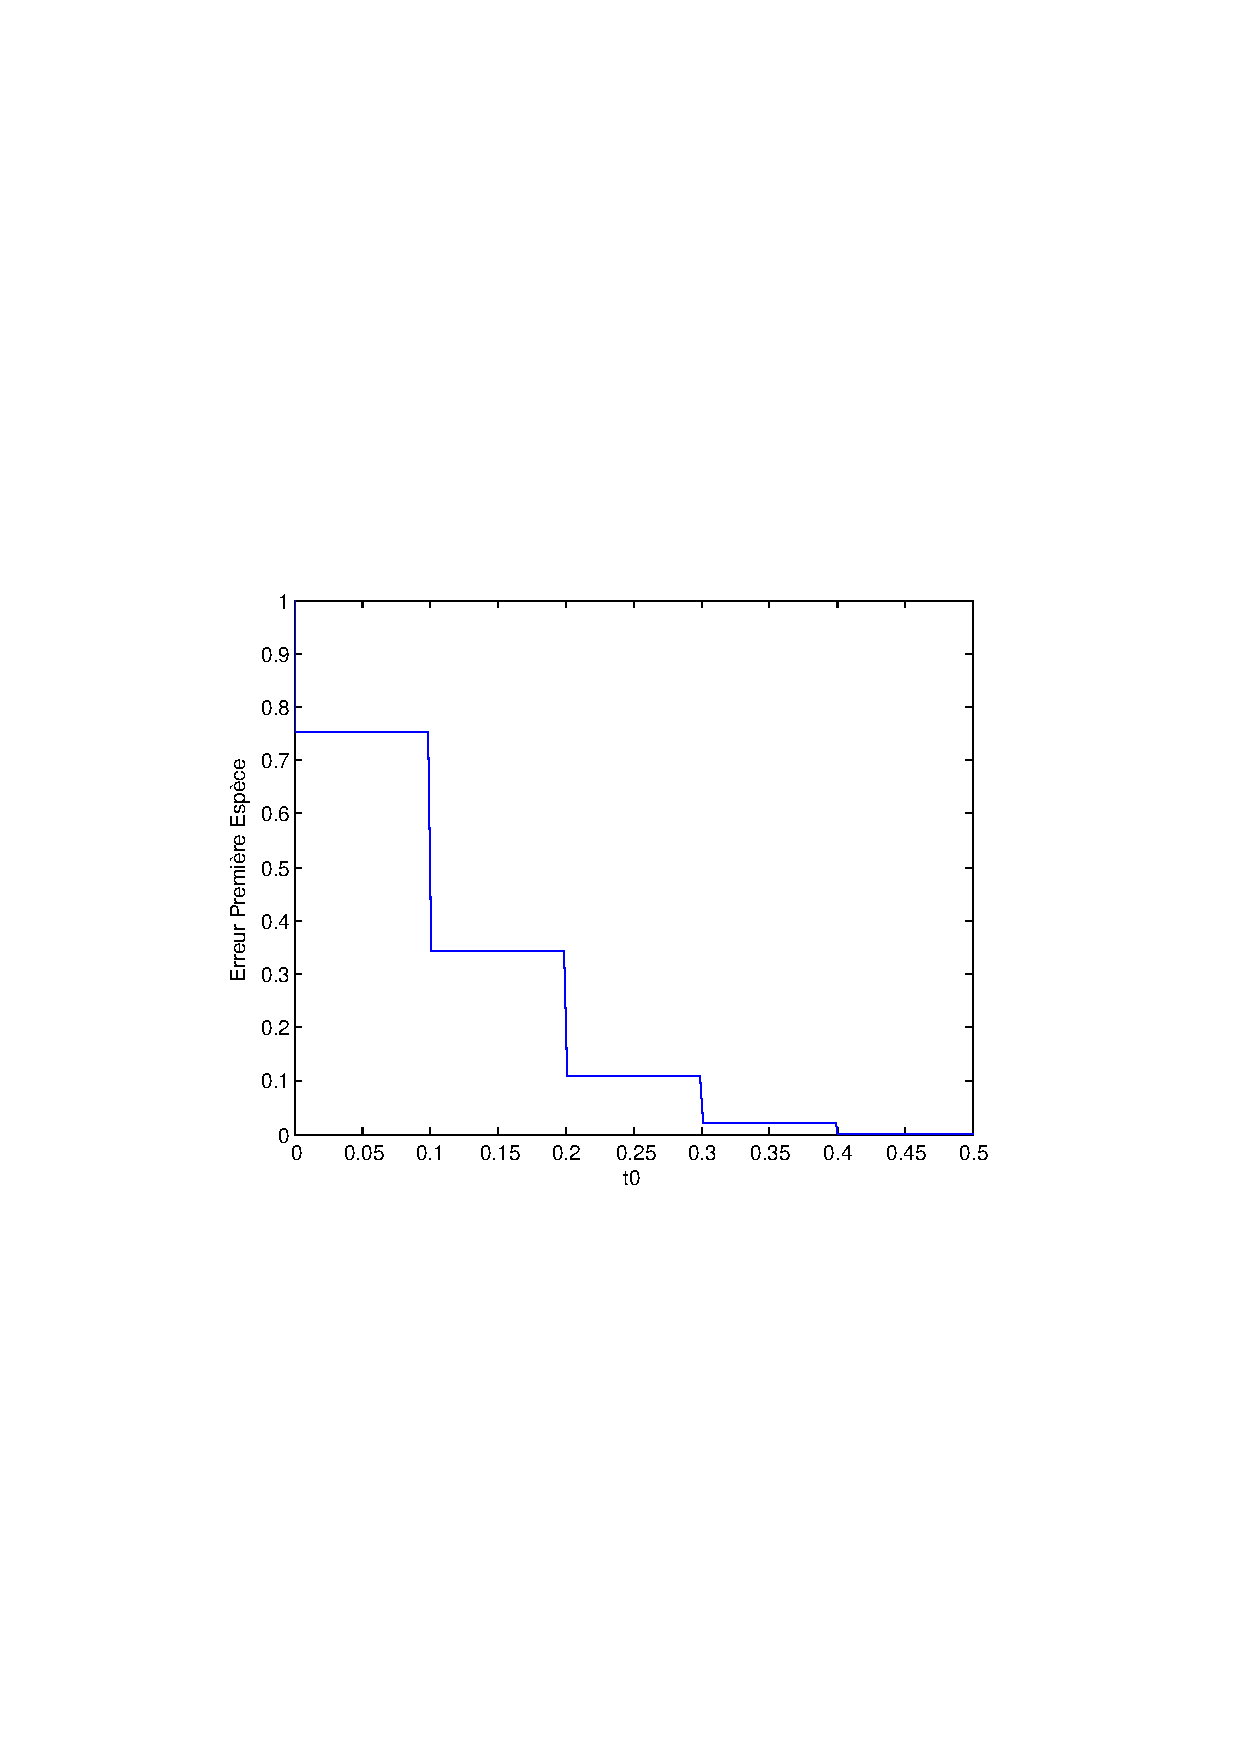
\includegraphics[width=0.7\textwidth]{ErreurPremiereEspece}\\
  \caption{Erreur de Première Espèce en fonction de la valeur critique: fonction décroissante de $t_0$ !}
\end{figure}

\end{frame}


\begin{frame}
\frametitle{Retour à l'exemple}
\begin{itemize}
\item Sous $\PP_\theta$, $n \hat{\theta}(Z)= \sum_{i=1}^n Z_i$ suit une loi binomiale de paramètre de succès $\truetheta$.
En notant $\binom_{n,\truetheta}$ la fonction
de répartition de la loi binomiale,
\begin{multline*}
\PP_\truetheta( |\hat{\theta}(Z) - 1/2| \leq t_0 ) \\
= \{\binom_{n,\truetheta}(n(1+t_0)/2) - \binom_{n,\truetheta}(n(1-t_0)/2)  \eqsp.
\end{multline*}
\item \alert{Erreur de seconde espèce}: pour une valeur critique fixée:
\begin{multline*}
\truetheta \mapsto \PP_{\truetheta}(|\hat{\theta}(Z) - 1/2| \leq t_0) \\=
\binom_{n,1/2}(n(1+t_0)/2) - \binom_{n,1/2}(n(1-t_0)/2)  \}
\end{multline*}
\end{itemize}
\end{frame}


\begin{frame}
\frametitle{Erreur de seconde espèce}
\begin{figure}
  \centering
  % Requires \usepackage{graphicx}
  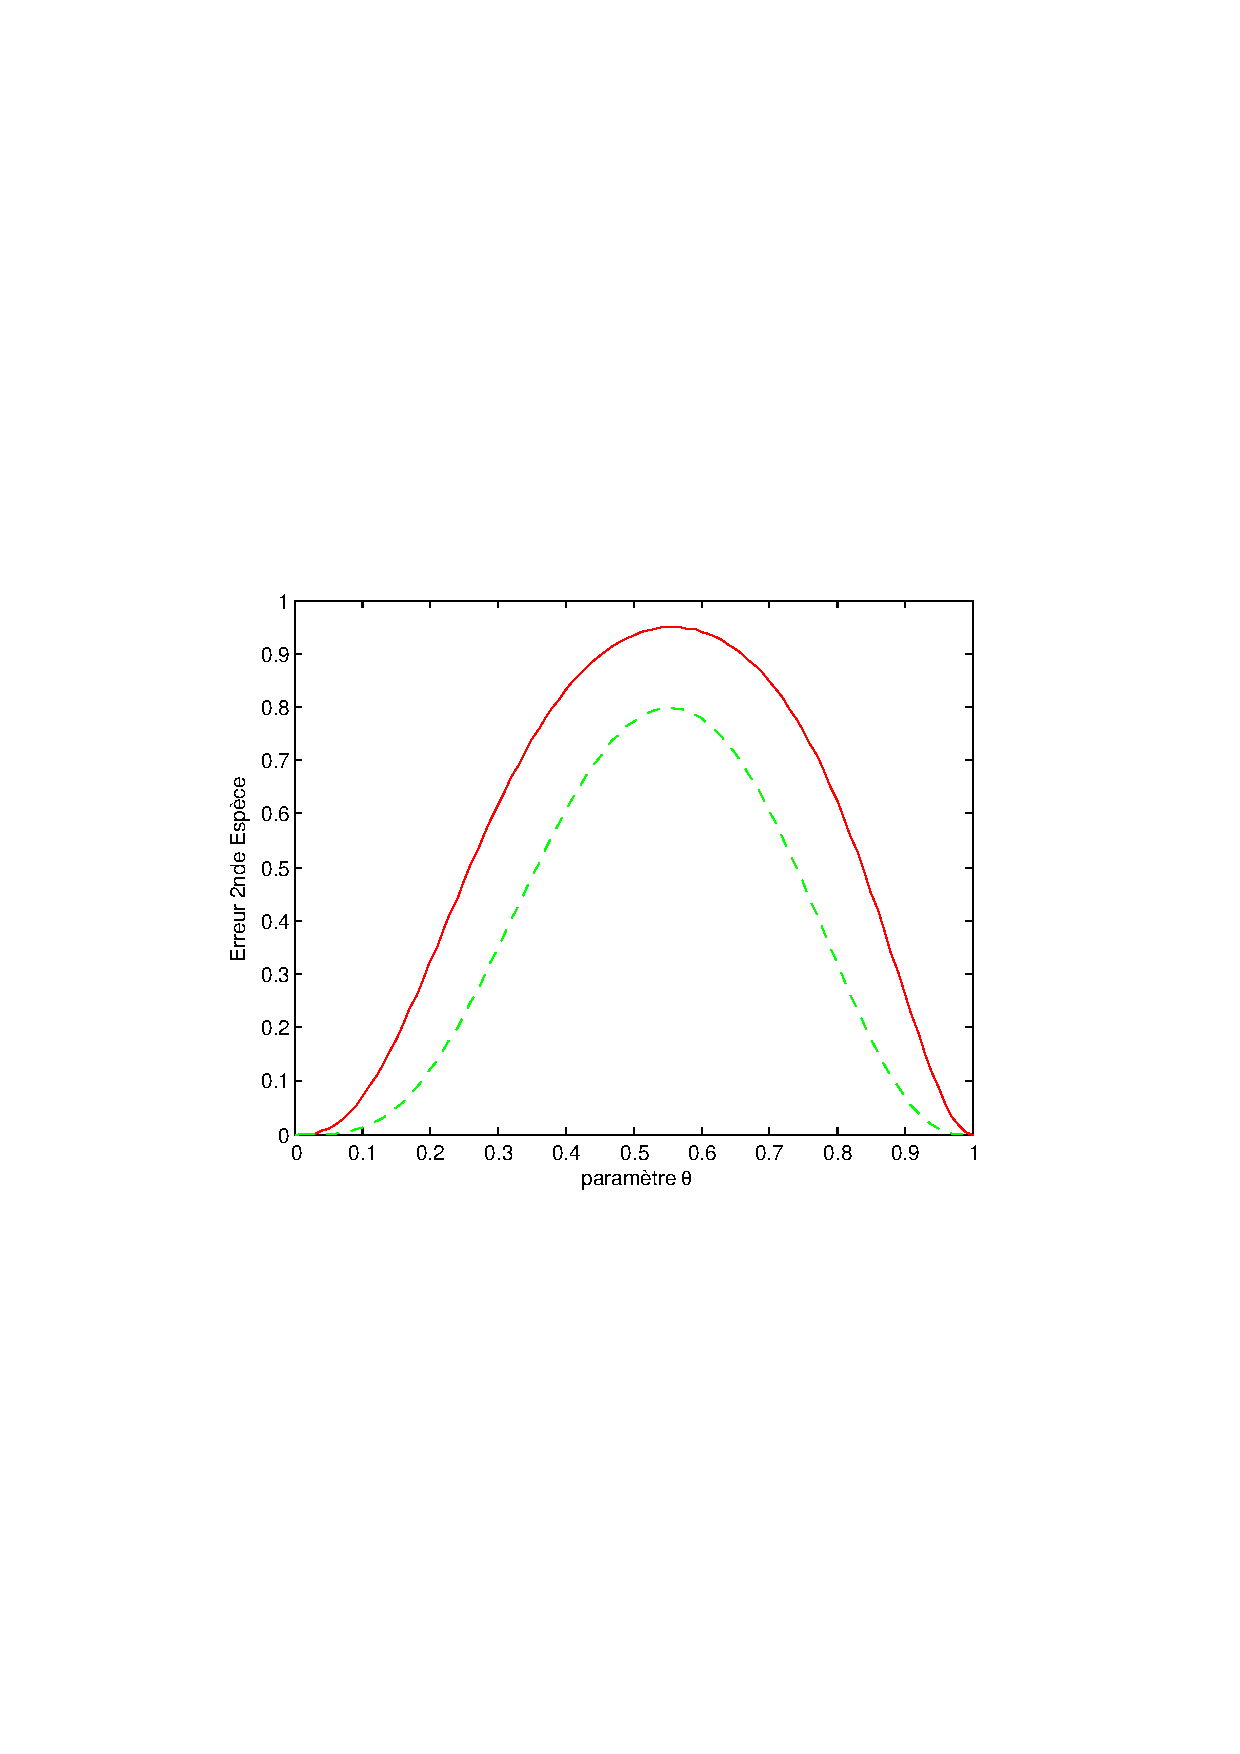
\includegraphics[width=0.6\textwidth]{Erreur2ndEspece}\\
  \caption{Erreur de deuxième Espèce en fonction du paramètre $\truetheta \in \Theta_1= \ccint{0,1}\setminus \{1/2\}$
  pour deux valeurs du seuil critique: $t_0=0.3$, Erreur 1ere espèce  0.0654 et $t_0= 0.2$, Erreur 1ère espèce 0.22 }
\end{figure}
\end{frame}

\begin{frame}
\frametitle{Puissance du test}
\begin{figure}
  \centering
  % Requires \usepackage{graphicx}
  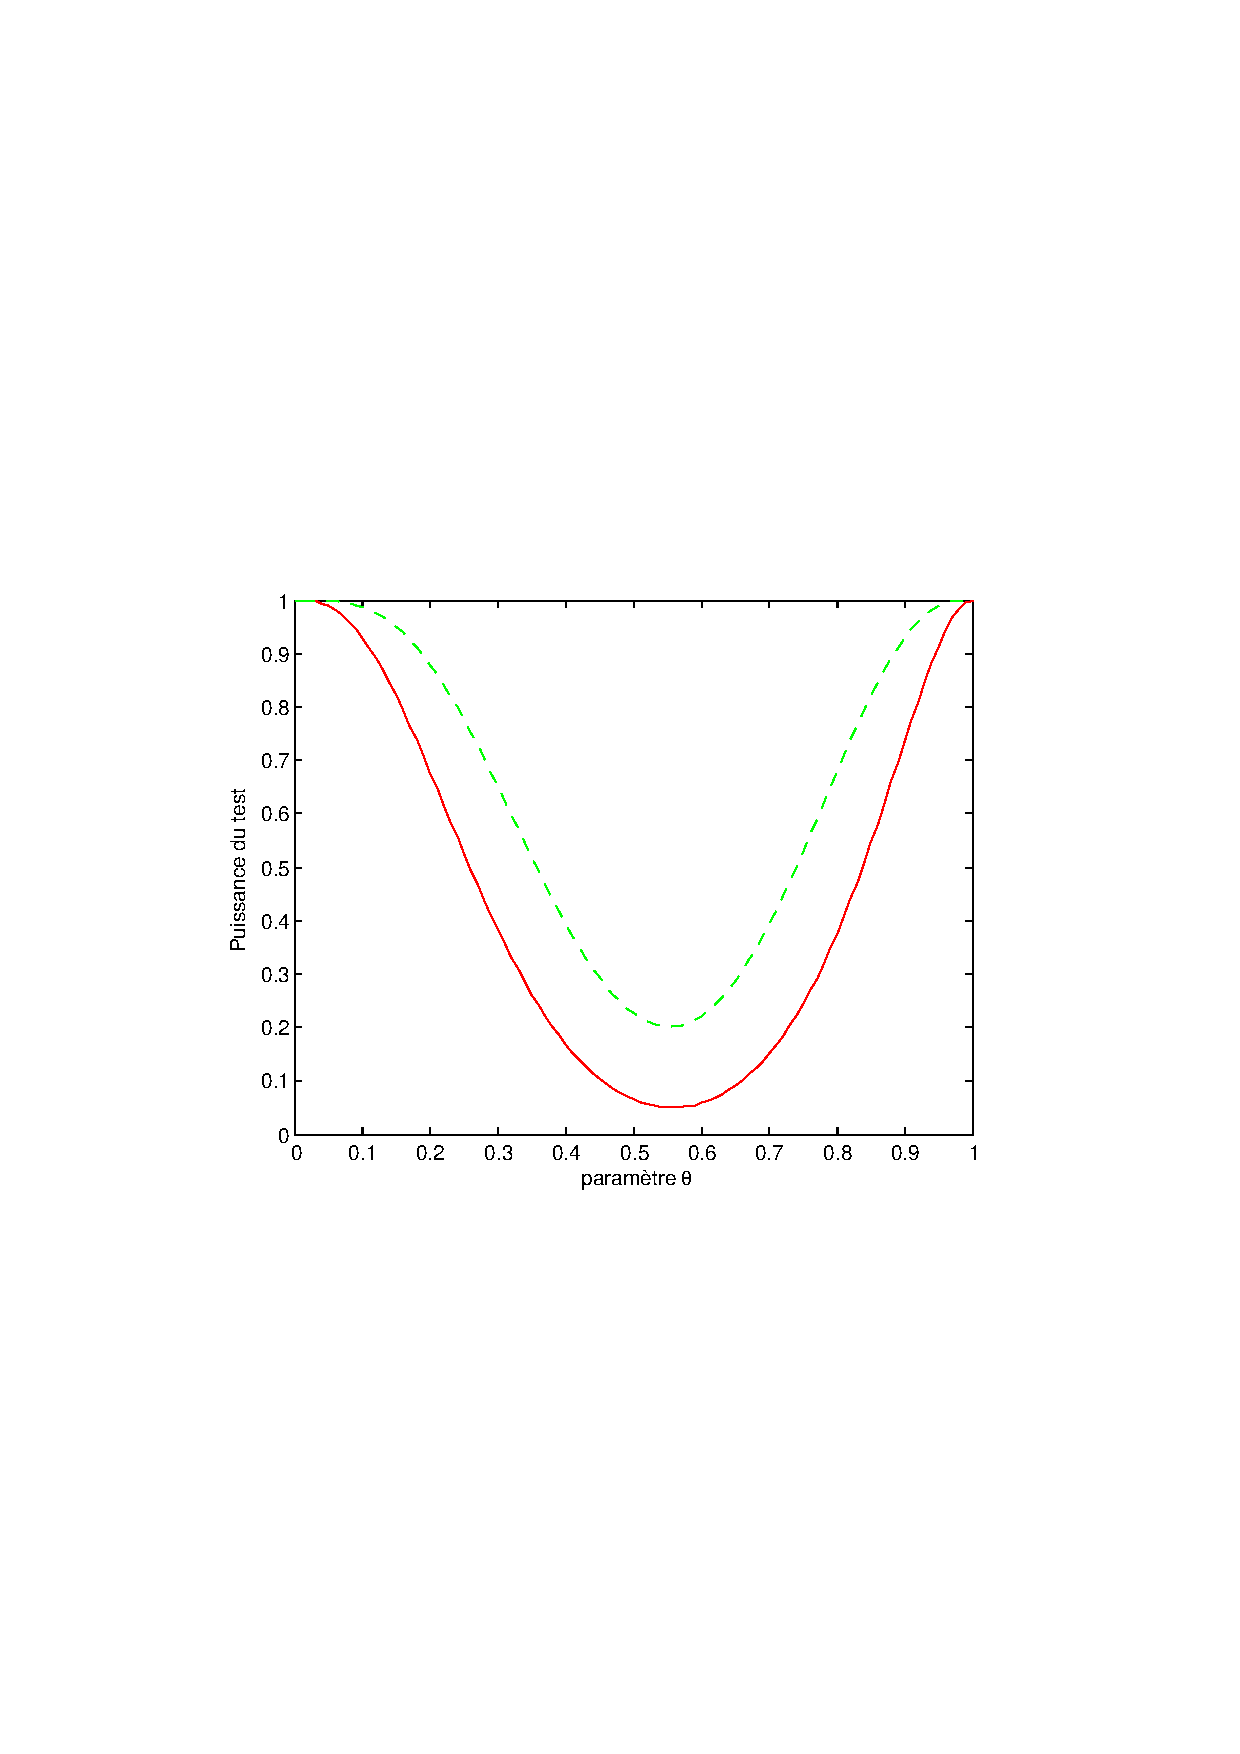
\includegraphics[width=0.6\textwidth]{Puissance}\\
  \caption{Puisance du test en fonction du paramètre $\truetheta \in \Theta_1= \ccint{0,1}\setminus \{1/2\}$
  pour deux valeurs du seuil critique: $t_0=0.3$. Erreur 1ere espèce: 0.0654 et $t_0= 0.2$, Erreur 1ère espèce: 0.22 }
\end{figure}
\end{frame}

\begin{frame}
\frametitle{Erreur 1ère espèce / Puissance}
\begin{figure}
  \centering
  % Requires \usepackage{graphicx}
  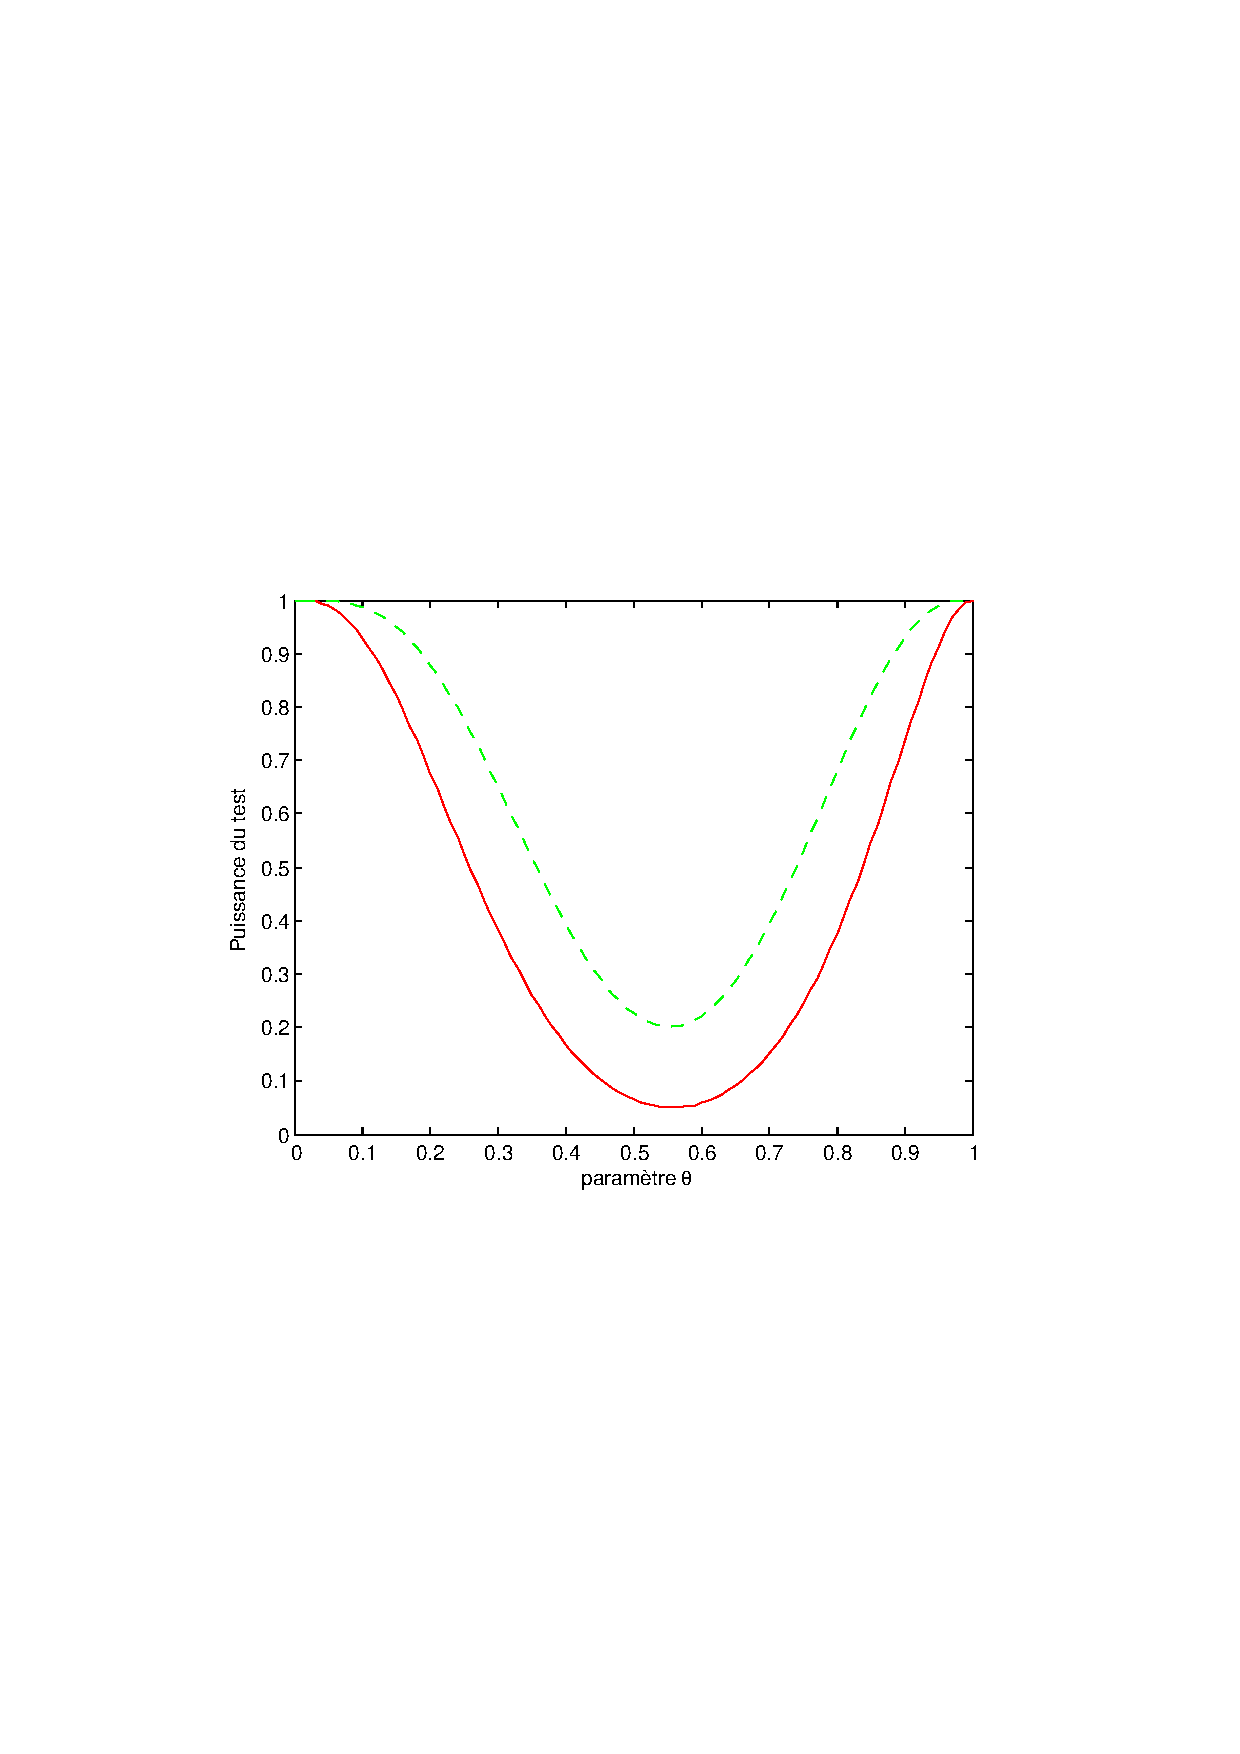
\includegraphics[width=0.6\textwidth]{Puissance}\\
  \caption{Erreur de première espèce / puisance pour une contre-alternative fixée $\theta_1=0.75$ pour différentes valeurs du seuil critique $t_0$. }
\end{figure}
\end{frame}

\begin{frame}
\frametitle{Conclusion provisoire}
\begin{itemize}
\item Un  bon test  $\varphi$ devrait garantir \alert{ simultanément} des erreurs de première et seconde espèce \alert{petites}.
\item Mais il faut réaliser un compromis entre erreur de 1ère espèce et erreur de 2nde espèce (ou de façon équivalente entre erreur de 1ère espèce et puissance).
\item \alert{Question:} comment aborder la notion d'optimalité et comment construire une procédure de test satisfaisante ?
\end{itemize}
\end{frame}



\begin{frame}
\frametitle{Définition formelle}
\begin{itemize}
\item \underline{Situation} : ${\mathcal E} = \big({\mathcal Z}, \mathfrak{Z}, \{\PP_\truetheta, \truetheta \in \Theta\}\big)$ engendrée par l'observation $Z$.
\item \alert{Hypothèse nulle et alternative} : $\Theta_0 \subset \Theta$ et $\Theta_1 = \Theta \setminus \Theta_0$
\end{itemize}
\begin{df}[Test simple] Un test (simple) de l'hypothèse nulle $H_0: \truetheta \in \Theta_0$ contre l'alternative $H_1:\truetheta \in \Theta_1$ est une statistique $\varphi  = \varphi(Z) \in \{0,1\}$.
 (Fonction d') \alert{erreur de première espèce} :
$$\truetheta \in \Theta_0 \leadsto \PP_\truetheta\big[\varphi(Z) = 1\big]$$
 (Fonction d') \alert{erreur de seconde espèce}
$$\truetheta \in \Theta_1 \leadsto \PP_\truetheta \big[\varphi(Z) = 0\big] = 1- \text{\alert{puissance}}_\varphi(\truetheta).$$
\end{df}
\end{frame}




\begin{frame}
\frametitle{Principe de Neyman}
\begin{itemize}
\item
On  \alert{disymétrise}  les hypothèses $H_0$ et $H_1$
: $H_0$ est  plus importante  que $H_1$ dans le sens suivant : on \alert{ impose} une \alert{erreur de première espèce prescrite}.
\end{itemize}
\begin{df}
Pour $\alpha \in [0,1]$, un test $\varphi = \varphi_\alpha$ de l'hypothèse nulle $H_0:\truetheta \in \Theta_0$ contre une alternative $H_1$ est de niveau $\alpha$ si
$$\sup_{\truetheta \in \Theta_0}\PP_\truetheta\big[\varphi_\alpha = 1\big] \leq \alpha.$$
\end{df}
\begin{itemize}
\item Un test de niveau $\alpha$ ne dit \alert{rien} sur l'erreur de seconde espèce (comportement sur l'alternative).
\end{itemize}
\end{frame}


\begin{frame}
\frametitle{Principe de Neyman (cont.)}
\begin{itemize}
\item Choix de la  disymétrisation  = choix de modélisation.
%Cas évident (dépistage d'une maladie), cas moins évident (détection de missile, efficacité d'un médicament).
\item \underline{\alert{Principe de Neyman}}  : $\alpha \in (0,1)$, parmi les test de niveau $\alpha$, chercher celui (ou ceux) ayant \alert{une erreur de seconde espèce minimale}.
\end{itemize}
\begin{df}
Un test de niveau $\alpha$ est dit \alert{Uniformément Plus Puissant} (UPP) si son erreur de seconde espèce est minimale parmi celles des tests de niveau $\alpha$.
\end{df}
\begin{itemize}
\item Pour le cas d'une \alert{hypothèse simple} contre une \alert{alternative simple}, un test UPP existe.
\end{itemize}
\end{frame}

\begin{frame}
\frametitle{Règle de décision randomisée}
\begin{itemize}
\item Pour toute valeur de l'observation $z$, la règle de décision choisit alternative avec une probabilité $\varphi(z)$ et l'hypothèse nulle avec la probabilité $1 - \varphi(z)$.
\item Une procédure de test randomisée est \alert{entièrement spécifiée} par la donnée de la \alert{fonction critique} du test $\varphi: z \to \varphi(z) \in [0,1]$. Si $\varphi$ prend simplement les valeurs $0$ et $1$, on obtient un test non randomisé.
\item La \alert{probabilité de rejet} est donnée, pour tout $\theta \in \Theta$, par $\PE_\theta[\varphi(Z)]$.
\end{itemize}
\end{frame}

\begin{frame}
\frametitle{Principe de Neyman-Pearson}
Le problème revient donc à maximiser la \alert{puissance du test}
\[
\puissance(\truetheta)= \PE_{\theta}[\varphi(Z)] \eqsp, \truetheta \in \Theta_1
\]
sous la contrainte que le niveau du test soit inférieure à $\alpha$
\[
\PE_\theta[\varphi(Z)] \leq \alpha
\]
\end{frame}

\subsection{Lemme de Neyman-Pearson}

\begin{frame}
\frametitle{Un cas élémentaire}
\begin{itemize}
\item Supposons que $\Theta_0 = \{\theta_0\}$ et $\Theta_1=\{ \theta_1 \}$.
\item On note $p_0(z)= f(\theta_0,z)$ et $p_1(z)= f(\theta_1,z)$ les densités des lois $\PP_{\theta_0}$ et $\PP_{\theta_1}$ par rapport à une mesure de domination $\mu$ (existe toujours)
\end{itemize}
\begin{theorem}[Existence d'un test de niveau $\alpha$]
 Pour tester $H_0: \{\theta = \theta_0\}$ contre l'alternative $H_1 : \{\theta = \theta_1\}$, il existe un test $\varphi$ et une constante $c_\alpha$ telle que
$$
\PE_{\theta_0}[\phi(Z)]= \alpha
$$
et
\[
\varphi(z)=
\begin{cases}
1 & \text{quand $p_1(z) > c_\alpha p_0(z)$} \\
0 & \text{quand $p_0(z) < c_\alpha p_1(z)$}
\end{cases}
\]
\end{theorem}
\end{frame}

\begin{frame}
\frametitle{Preuve}
\begin{itemize}
\item Soit $\alpha(c)= \PP_0( p_1(Z) > c p_0(Z))$, qui est la probabilité que la variable aléatoire $p_1(Z)/p_0(Z)$ soit strictement plus grande que $c$ (il suffit de se placer sur l'événement $\{p_0(Z) > 0 \}$).
\item $c \mapsto \alpha(c)$ est donc décroissante, continue à droite et admet des limites à gauches ($c \mapsto 1 - \alpha(c)$ est une fonction de répartition !)
$$
\alpha(c^-) - \alpha(c) = \PP_0( p_1(Z)/p_0(Z) = c) \eqsp, \alpha(-\infty)= 1, \alpha(+\infty)=0
$$
\end{itemize}
\end{frame}

\begin{frame}
\frametitle{Preuve}
\begin{itemize}
\item Pour tout $\alpha \in \ooint{0,1}$, il existe $c_\alpha$ tel que $\alpha(c_\alpha) \leq \alpha \leq \alpha(c_\alpha^-)$.
\item On considère le test $\varphi_\alpha$ définit par
$$
\varphi_\alpha(z)
=
\begin{cases}
1 & \quad \text{quand $p_1(z) > c_\alpha p_0(z)$} \\
\frac{\alpha - \alpha(c_\alpha)}{\alpha(c_\alpha^-)-\alpha(c_\alpha)} & \text{quand $p_1(z) = c_\alpha p_0(z)$} \\
0  & \quad \text{quand $p_1(z) < c_\alpha p_0(z)$}
\end{cases}
$$
La seconde ligne a un sens seulement si $\alpha(c_\alpha^-)  > \alpha(c_\alpha)$.
\item Le niveau de $\phi$ est donné par
\begin{align*}
\PE_0[\varphi(Z)] &= \PP_0 \left( \frac{p_1(Z)}{p_0(Z)} > c_\alpha \right) + \frac{\alpha-\alpha(c_\alpha)}{\alpha(c_\alpha^-)-\alpha(c_\alpha)}
\PP_0\left( \frac{p_1(Z)}{p_0(Z)} = c_\alpha \right) \\
&= \alpha
\end{align*}
\end{itemize}
\end{frame}


\begin{frame}
\frametitle{Test le plus puissant}
\begin{theorem}
Un test $\varphi$ vérifiant
$$
\PE_{\theta_0}[\phi(Z)]= \alpha
$$
et
\[
\varphi(z)=
\begin{cases}
1 & \text{quand $p_1(z) > c_\alpha p_0(z)$} \\
0 & \text{quand $p_0(z) < c_\alpha p_1(z)$}
\end{cases}
\]
est \alert{uniformément le plus puissant} pour tester l'hypothèse nulle $H_0: \{\theta = \theta_0\}$ contre l'alternative $H_1: \{\theta = \theta_1\}$.
\end{theorem}
\end{frame}

\begin{frame}
\frametitle{Preuve}
\only<1>{Soit $\varphi$ un test satisfaisant les conditions
$$
\PE_{\theta_0}[\phi(Z)]= \alpha
$$
et
\[
\varphi(z)=
\begin{cases}
1 & \text{quand $p_1(z) > c_\alpha p_0(z)$} \\
0 & \text{quand $p_0(z) < c_\alpha p_1(z)$}
\end{cases}
\]
et $\varphi^*$ un test de niveau $\PE_0[\varphi^*(Z)] \leq \alpha$}
\only<2>{
\begin{itemize}
\item On note $S^+= \{z : \varphi(z) - \varphi^*(z) > 0\}$ et $S^-=\{ z: \varphi(z) - \varphi^*(z) < 0\}$.
\item Pour $z \in S^+$, $\phi(z) > 0$ et donc $p_1(z) \geq c_\alpha p_0(z)$.
\item Pour $z \in S^-$, $\phi(z) < 1$ et donc $p_1(z) \leq c_\alpha p_0(z)$.
\item Par conséquent:
$$
\int (\varphi - \varphi^*) (p_1 - c_\alpha p_0) \rmd \mu \geq 0
$$
\end{itemize}
}
\only<3>
{Comme
$$
\int (\varphi - \varphi^*) (p_1 - c_\alpha p_0) \rmd \mu \geq 0
$$
Nous avons
$$
\int (\varphi - \varphi^*) (p_1 - c_\alpha p_0) \rmd \mu \geq c_\alpha \int (\varphi - \varphi^*) (p_1 - c_\alpha p_0) \rmd \mu \geq 0 \eqsp.
$$
}
\end{frame}

\begin{frame}
\frametitle{Puissance d'un test U.P.P}
\begin{lemma}
Notons $\puissance$ la puissance du test U.P.P de niveau $\alpha$ du test $H_0= \{\theta = \theta_0\}$ contre l'alternative $H_1= \{\theta=\theta_1\}$. Alors $\alpha \leq \beta$ avec égalité si $\PP_{\theta_0}= \PP_{\theta_1}$.
\end{lemma}
\begin{proof}
Comme le test $\varphi(z) \equiv \alpha$ a un niveau $\alpha$, nous avons $\alpha \leq \beta$.
\end{proof}
\end{frame}

\begin{frame}
\frametitle{Exemple de mise en oeuvre}
\begin{itemize}
\item On observe
$$Z=(X_1,\ldots, X_n) \sim_{\text{i.i.d.}} {\mathcal N}(\truetheta, 1).$$
\item \alert{Construction du test de N-P.} de $H_0:\truetheta = \truetheta_0$ contre $H_1:\truetheta = \truetheta_1$, avec $\truetheta_0 < \truetheta_1$.
\item \alert{Mesure dominante} $\mu^n=\;$mesure de Lebesgue sur $\R^n$ et
$$f(\truetheta, Z)=\tfrac{1}{(2\pi)^{n/2}}\exp\big(-\frac{1}{2}\sum_{i = 1}^n X_i^2+n\truetheta\overline{X}_n-\frac{n\truetheta^2}{2}\big).$$
\item \alert{Rapport de vraisemblance}
$$\frac{f(\truetheta_1,Z)}{f(\truetheta_0,Z)} = \exp\big(n(\truetheta_1-\truetheta_0)\overline{X}_n-\frac{n}{2}(\truetheta_1^2-\truetheta_0^2)\big).$$
\end{itemize}
\end{frame}

\begin{frame}
\frametitle{Exemple (cont.)}
\begin{itemize}
\item \alert{Zone de rejet} du test de N-P. :
\begin{align*}
& \big\{f(\truetheta_1,Z) >  cf(\truetheta_0,Z)\big\}\\
  =& \big\{n(\truetheta_1-\truetheta_0)\overline{X}_n-\frac{n}{2}(\truetheta_1^2-\truetheta_0^2) > \log c\big\} \\
 =& \big\{\overline{X}_n > \frac{\truetheta_0+\truetheta_1}{2}+\tfrac{\log c}{n(\truetheta_0-\truetheta_1)}\big\}.
\end{align*}
\item \alert{Choix de $c$}. On résout
$$\PP_{\truetheta_0}\big[\overline{X}_n > \tfrac{1}{2}(\truetheta_0+\truetheta_1)+\tfrac{\log c}{n(\truetheta_0-\truetheta_1)}\big]=\alpha.$$
\item \alert{Approche standard} : on raisonne sous $\PP_{\truetheta_0}$. On a
$$\overline{X}_n = \truetheta_0 + \frac{1}{\sqrt{n}}\xi^{n,\truetheta_0},$$
où $\xi^{n,\truetheta_0}$ est une gaussienne standard ${\mathcal N}(0,1)$ sous $\PP_{\truetheta_0}$ \alert{mais pas sous une autre probabilité $\PP_\truetheta$ si $\truetheta \neq \truetheta_0$!}
\end{itemize}
\end{frame}

\begin{frame}
\frametitle{Exemple (fin)}
\begin{itemize}
\item \alert{Résolution de}
$$\PP_{\truetheta_0}\big[\truetheta_0 + \frac{1}{\sqrt{n}}\xi^{n,\truetheta_0} > \frac{1}{2}(\truetheta_0+\truetheta_1)+\frac{\log c}{n(\truetheta_0-\truetheta_1)}\big]=\alpha.$$
\item \alert{Equivalent à}
$\PP_{\truetheta_0}\big[\xi^{n\truetheta_0} > \frac{\sqrt{n}}{2}(\truetheta_1-\truetheta_0)+\frac{1}{\sqrt{n}}\frac{\log c}{\truetheta_0-\truetheta_1}\big]=\alpha,$
soit
$$\frac{\sqrt{n}}{2}(\truetheta_1-\truetheta_0)+\frac{1}{\sqrt{n}}\frac{\log c}{\truetheta_0-\truetheta_1}=\Phi^{-1}(1-\alpha),$$
où $\Phi(x) = \int_{-\infty}^x \rme^{-u^2/2}\tfrac{du}{\sqrt{2\pi}}$.
\item \alert{Conclusion}
$$\boxed{c_\alpha = \exp\big(n\frac{(\truetheta_1-\truetheta_0)^2}{2}+\sqrt{n}(\truetheta_0-\truetheta_1)\Phi^{-1}(1-\alpha)\big)}$$
\end{itemize}
\end{frame}


\begin{frame}
\frametitle{p-valeur}
\begin{itemize}
\item Supposons que sous $\PP_0$, la distribution du rapport de vraisemblance $p_1(Z)/p_0(Z)$ est continue. Le test U.P.P.
de niveau $\alpha$ est non-randomisé et rejette l'hypothèse nulle si $p_1(Z)/p_0(Z) > k$, où $k$ est choisi de façon à ce que
\[
\PP_0 ( p_1(Z)/ p_0(Z) \geq k) = \alpha.
\]
\item Lorsque l'on fait fait varier le niveau $\alpha$, on obtient ainsi une famille de régions de réjections, $\{\zreject_\alpha\}_{\alpha \in \ccint{0,1}}$, qui sont dans de nombreux cas d'intérêt emboitées
    $$
    \zreject_\alpha \subset \zreject_{\alpha'} \quad \text{si $\alpha < \alpha'$}.
    $$
\end{itemize}
\end{frame}


\begin{frame}
\frametitle{p-valeur}
\begin{itemize}
\item Lorsque l'on fait fait varier le niveau $\alpha$, on obtient ainsi une famille de régions de réjections, $\{\zreject_\alpha\}_{\alpha \in \ccint{0,1}}$, qui sont dans de nombreux cas d'intérêt emboitées
    $$
    \zreject_\alpha \subset \zreject_{\alpha'} \quad \text{si $\alpha < \alpha'$}.
    $$
\item Lorsque cette condition est satisfaite, il est intéressant de déterminer non seulement si le test est accepté ou rejeté à un niveau de signification donné, mais aussi de déterminer \alert{le plus petit niveau de signification} auquel l'hypothèse serait rejetée.
\end{itemize}
\end{frame}

\begin{frame}
\frametitle{p-valeur}
\begin{definition}[p-valeur]
La $p$-valeur d'un test pour une observation $Z$ donnée est le plus petit niveau de signification auquel le test serait rejeté
$$
\hat{p}(Z)= \inf\{ \alpha: Z \in S_\alpha\}.
$$
\end{definition}
\begin{itemize}
\item Une petite $p$-valeur suggère que l'observation contredit l'hypothèse.
\item Une grande $p$-valeur s'interprète en faveur de ne pas vouloir rejeter l'hypothèse de base.
\end{itemize}
\end{frame}

\begin{frame}
\frametitle{Bilan provisoire}
\begin{itemize}
\item Si l'on accepte \alert{le principe de Neyman}, on sait résoudre le problème à deux points.
\item Que faire si l'hypothèse nulle $H_0$ ou l'alternative $H_1$ sont \alert{composites} ?
\begin{itemize}
\item On peut proposer des extensions si l'on dispose de structures particulières sur la vraisemblance du modèle (Poly. Ch. 7.3, hors programme).
\item On sait dire \alert{ beaucoup de choses} dans le cas gaussien.
\end{itemize}
\item \alert{ Critique méthodologique de l'approche de Neyman} $\leadsto$ notion de $p$-valeur.
\end{itemize}
\end{frame}





\section{Tests gaussiens}

\subsection{Tests sur la moyenne}

\begin{frame}
\frametitle{Tests gaussiens incontournables}
\begin{itemize}
\item On observe
$$\bY=(Y_1,\ldots, Y_n) \sim {\mathcal N}(\mu, \sigma^2 \text{Id}_n).$$
\item \underline{\alert{Test sur la moyenne, variance connue}}
$$H_0:\mu \leq \mu_0\;\;\;\text{contre}\;\;\;H_1:\mu > \mu_0$$
\item \alert{ Principe} on estime $\mu$ et on rejette $H_0$ si l'estimateur est  plus grand  que $\mu_0$.
$${\mathcal R}(c_\alpha) = \big\{\overline{Y}_n - \mu_0 \geq c_\alpha\big\},\;\;\;c_\alpha\;\;\text{à déterminer}.$$
\item On choisit $c_\alpha$ de sorte que
$$\sup_{\mu \leq \mu_0}\PP_\mu\big[{\mathcal R}(c_\alpha)\big] \leq \alpha.$$
\item Il y a \alert{plusieurs choix possibles}. On fait le choix rendant  ${\mathcal R}(c_\alpha)$ \alert{  maximale}.
%\item On a \alert{seulement} optimalité parmi la classe de test de zone de rejet de la forme ${\mathcal R}(c), c >0$ sans outil supplémentaire.
\end{itemize}
\end{frame}

\begin{frame}
\frametitle{Calcul de $c_\alpha$}
\begin{itemize}
\item \alert{Majoration de l'erreur de première espèce}. Si $\mu \leq \mu_0$, on a
\begin{align*}
\PP_{\mu}\big[\overline{Y}_n - \mu_0 \geq c_\alpha\big] & = \PP_\mu\big[(\mu+\tfrac{\sigma}{\sqrt{n}}\xi^{n,\mu})-\mu_0 \geq c_\alpha\big] \\
& =   \PP_{\mu}\big[\tfrac{\sigma}{\sqrt{n}}\xi^{n,\mu} \geq c_\alpha + (\mu_0-\alert{\mu})\big] \\
& \leq \PP_{\mu}\big[\tfrac{\sigma}{\sqrt{n}}\xi^{n,\mu} \geq c_\alpha\big].
\end{align*}
où $\xi^{n,\mu}$ est, en loi sous $\PP_\mu$, une gaussienne standard.
\item \alert{ Petit miracle} : la loi de $\xi^{n,\mu}$ sous $\PP_\mu$ ne \alert{dépend pas de} $\mu$
% (on parle de statistique libre).
Donc
\begin{align*}
\PP_{\mu}\big[\tfrac{\sigma}{\sqrt{n}}\xi^{n,\mu} \geq c_\alpha\big] & =1-\Phi\big(\tfrac{\sqrt{n}}{\sigma}c_\alpha\big) \\
& \stackrel{\text{on veut}}{\leq} \alpha.
\end{align*}
\item Le choix $c_{\alpha,n} = \tfrac{\sigma}{\sqrt{n}}\Phi^{-1}(1-\alpha)$ conduit à la zone de rejet ${\mathcal R}(c_\alpha)$ \alert{maximale}.
\end{itemize}
\end{frame}

\begin{frame}
\frametitle{Contrôle de l'erreur de seconde espèce}
\begin{itemize}
\item On a construit un test de niveau $\alpha$ parmi une classe \alert{donnée a priori} de tests basés sur un estimateur  raisonnable, de sorte que l'on ait une zone de rejet maximale. Désormais, $c_{\alpha, n}$ est \alert{fixé}.
\item On \alert{évalue à la main} l'erreur de seconde espèce ou la \alert{fonction de puissance}
\begin{align*}
\mu \in (\mu_0,+\infty) & \leadsto \PP_\mu\big[\overline{Y}_n - \mu_0 < c_{\alpha,n}\big] \\
&= 1 - {\text{puissance du test au point }}\mu
\end{align*}
\item \alert{Montrer que} pour tout $\mu > \mu_0$, on a $\PP_\mu\big[\overline{Y}_n - \mu_0 < c_{\alpha,n}\big] \rightarrow 0$ lorsque $n\rightarrow \infty$.
\item Pour l'optimalité dans un sens plus fort, il faut \alert{ d'autres outils}.
\end{itemize}
\end{frame}

\begin{frame}
\frametitle{Autres tests classiques gaussiens}
\begin{itemize}
%\item \underline{\alert{Test sur la moyenne et la  variance}}.
\item \alert{Ingrédient principal} :
$$s_n^2:=\frac{1}{n-1}\sum_{i = 1}^n (Y_i-\overline{Y}_n)^2 = \frac{n}{n-1}\big(\widehat \sigma^2_n\big)^{{\tt mv}}$$
alors
$$(n-1)\frac{s_n^2}{\sigma^2} \sim \chi^2(n-1)$$
et
$$\frac{\sqrt{n}(\overline{Y}_n-\mu)}{s_n} \sim \text{Student}(n-1)$$
et ces variables sont \alert{pivotales} : leur loi ne dépend pas de $\mu,\sigma^2$ sous $\PP_{\mu,\sigma^2}$.
\item Les lois du \alert{$\chi^2$} et de \alert{Student} (à $k$ degrés de liberté) sont classiques et s'étudient indépendamment.
\end{itemize}
\end{frame}

%\begin{frame}
%\frametitle{Tests sur la moyenne}
%\begin{itemize}
%\item On teste \alert{$H_0 : \mu \leq \mu_0$ contre $H_1: \mu > \mu_0$}. Un test de niveau $\alpha$ : donné par
%$${\mathcal R}_\alpha = \big\{T(\bY)>q_{1-\alpha, n-1}^{\mathfrak T}\big\}$$
%où
%$$T(Y)  = \frac{\sqrt{n}(\overline{Y}_n-\mu_0)}{s_n}$$
%%et $q_{1-\alpha, n-1}^{\mathfrak{T}}$ = quantile d'ordre $1-\alpha$ de la loi de Student à $n-1$ degrés de liberté :
%où
%$$\PP\big[\text{Student}_{n-1} > q_{1-\alpha, n-1}^{\mathfrak{T}}\big]=\alpha$$
%\item On teste \alert{ $H_0 : \mu = \mu_0$ contre $H_1:\mu \neq \mu_0$}. Un test de niveau $\alpha$: donné par
%${\mathcal R}_\alpha = \big\{\big|T(\bY)\big| > q_{1-\alert{\alpha/2}, n-1}^{\mathfrak{T}}\big\}$.
%\end{itemize}
%\end{frame}
%\subsection{Tests sur la variance}
%\begin{frame}
%\frametitle{Test sur la variance}
%\begin{itemize}
%\item On teste \alert{ $H_0:\sigma^2 \leq \sigma_0^2$ contre $H_1:\sigma^2 > \sigma_0^2$}. Un test de niveau $\alpha$ : donné par
%$${\mathcal R}_\alpha = \big\{V(\bY)>q_{1-\alpha,n-1}^{\chi^2}\big\},$$
%où
%$$V(\bY) = \frac{1}{\sigma_0^2}\sum_{i = 1}^n (Y_i - \overline{Y})^2$$
%et
%$$\PP\big[\text{Chi-deux}_{n-1} > q_{1-\alpha,n-1}^{\chi^2}\big] = \alpha.$$
%\item \alert{Mêmes remarques méthodologiques} sur l'optimalité de ces tests que précédemment.
%\end{itemize}
%\end{frame}


\section{Compléments : $p$-valeur et liens entre tests et régions de confiance}

\begin{frame}
\frametitle{$p$-valeurs}
\begin{itemize}
\item \alert{Exemple} : on observe
$$X_1,\ldots, X_n\sim_{\text{i.i.d.}}{\mathcal N}(\mu,\sigma^2),\;\;\;\sigma^2\;\;\text{connu}.$$
\item \alert{Objectif}: tester $H_0:\mu=0$ contre $H_1:\mu\neq 0$.
\item Au niveau $\alpha=5\%$, on rejette si
$$\big| \overline{X}_n \big| > \frac{\phi^{-1}(1-\alpha/2)}{\sqrt{n}}$$
\item \alert{Application numérique} : $n=100$, $\overline{X}_{100}=0.307$. On a $\frac{\phi^{-1}(1-0.05/2)}{\sqrt{100}} \approx 0.196$. \alert{on rejette l'hypothèse...}.
%\item
\end{itemize}
\end{frame}

\begin{frame}
\frametitle{$p$-valeur (cont.)}
\begin{itemize}
\item \alert{Et pour un autre choix de $\alpha$ ?}. Pour $\alpha=0.01$, on a $\frac{\phi^{-1}(1-0.05/2)}{\sqrt{100}} \approx 0.256$. On rejette toujours... Pour $\alpha=0.001$, on a $\frac{\phi^{-1}(1-0.05/2)}{\sqrt{100}} \approx 0.329$. \alert{On accepte $H_0$ !}
\item Que penser de cette petite expérience ?
\begin{itemize}
\item En pratique, on a une observation une bonne fois pour toute (ici $0.307$) et on  choisit  $\alpha$... \alert{comment ?}
\item On ne veut pas $\alpha$ trop grand (trop de risque), mais en prenant $\alpha$ de plus en plus petit... on va \alert{ fatalement} finir par accepter $H_0$ !
\end{itemize}
\item Défaut de méthodologie inhérent au principe de Neyman (contrôle de l'erreur de première espèce).
\end{itemize}
\end{frame}


\begin{frame}
\frametitle{p-valeur}
\begin{itemize}
\item Quantité \alert{significative} : non par le niveau $\alpha$, mais le \alert{seuil de basculement de décision} : c'est la $p$-valeur ($p$-value) du test.
\end{itemize}
\begin{df}
Soit ${\mathcal R}_\alpha$ une famille de zones de rejet d'un test de niveau $\alpha$ pour une hypothèse $H_0$ contre une alternative $H_1$. Soit $Z$ l'observation associée à l'expérience. On a $Z \in \mathfrak{Z}$ et ${\mathcal R}_0 = \mathfrak{Z}$.
On appelle \alert{$p$-valeur du test} la quantité
$$p-\text{valeur}(Z) = \inf\{\alpha, Z \in {\mathcal R}_\alpha\}.$$
\end{df}
\end{frame}

\begin{frame}
\frametitle{Interprétation de la $p$-valeur}
\begin{itemize}
\item Une grande valeur de la $p$-valeur s'interprète en faveur de \alert{ne pas vouloir rejeter l'hypothèse}.
\item  Ne pas vouloir rejeter l'hypothèse  peut signifier deux choses :
\begin{itemize}
\item L'hypothèse est vraie
\item L'hypothèse est fausse \alert{ mais} le test n'est pas \alert{puissant} (erreur de seconde espèce \alert{grande}).
\end{itemize}
\item \alert{Souvent :} la $p$-valeur est la probabilité (sous $H_0$) que la statistique de test d'une expérience  copie  soit $\geq$ à la statistique de test observée.
\item \alert{Exemple du test du $\chi^2$ et de l'expérience de Mendel} (à suivre) %
\end{itemize}
\end{frame}



\end{document}

